\documentclass[a4paper,twoside,openright,makeidx,12pt]{book}
%\usepackage{draftcopy}
%$Id: macro.tex,v 1.10 2004/12/08 13:38:58 acary Exp $


%\usepackage{a4wide}
\textheight 25cm
\textwidth 16.5cm
\topmargin -1cm
%\evensidemargin 0cm
\oddsidemargin 0cm
\evensidemargin0cm
\usepackage{layout}


\usepackage{amsmath}
\usepackage{amssymb}
\usepackage{minitoc}
%\usepackage{glosstex}
\usepackage{colortbl}
\usepackage{hhline}
\usepackage{longtable}

%\usepackage{glosstex}
%\def\glossaryname{Glossary of Notation}
\def\listacronymname{Acronyms}

\usepackage[outerbars]{changebar}\setcounter{changebargrey}{20}
%\glxitemorderdefault{acr}{l}

%\usepackage{color}
\usepackage{graphicx,epsfig}
\graphicspath{{figure/}}
\usepackage[T1]{fontenc}
\usepackage{rotating}

%\usepackage{algorithmic}
%\usepackage{algorithm}
\usepackage{ntheorem}
\usepackage{natbib}


%\renewcommand{\baselinestretch}{2.0}
\setcounter{tocdepth}{2}     % Dans la table des matieres
\setcounter{secnumdepth}{3}  % Avec un numero.



\newtheorem{definition}{Definition}
\newtheorem{lemma}{Lemma}
\newtheorem{claim}{Claim}
\newtheorem{remark}{Remark}
\newtheorem{assumption}{Assumption}
\newtheorem{example}{Example}
\newtheorem{conjecture}{Conjecture}
\newtheorem{corollary}{Corollary}
\newtheorem{OP}{OP}
\newtheorem{problem}{Problem}
\newtheorem{theorem}{Theorem}


\newcommand{\CC}{\mbox{\rm $~\vrule height6.6pt width0.5pt depth0.25pt\!\!$C}}
\newcommand{\ZZ}{\mbox{\rm \lower0.3pt\hbox{$\angle\!\!\!$}Z}}
\newcommand{\RR}{\mbox{\rm $I\!\!R$}}
\newcommand{\NN}{\mbox{\rm $I\!\!N$}}

\newcommand{\Mnn}{\mathcal M^{n\times n}}
\newcommand{\Mnp}[2]{\ensuremath{\mathcal M^{#1\times #2}}}



\newcommand{\Frac}[2]{\displaystyle \frac{#1}{#2}}

\newcommand{\DP}[2]{\displaystyle \frac{\partial {#1}}{\partial {#2}}}

% c++ variables writting
\newcommand{\varcpp}[1]{\textit{#1}}
% itemize
\newcommand{\bei}{\begin{itemize}}
\newcommand{\ei}{\end{itemize}}

\newcommand{\ie}{i.e.}
\newcommand{\eg}{e.g.}
\newcommand{\cf}{c.f.}
\newcommand{\putidx}[1]{\index{#1}\textit{#1}}

\def\Er{{\rm I\! R}}
\def\En{{\rm I\! N}} 
\def\Ec{{\rm I\! C}}
 
\def\zc{\hat{z}}
\def\wc{\hat{w}}

\font\tete=cmr8 at 8 pt
\font\titre= cmr12 at 20 pt 
\font\titregras=cmbx12 at 20 pt

%----------------------------------------------------------------------
%                  Modification des subsubsections
%----------------------------------------------------------------------
\makeatletter
\renewcommand\thesubsubsection{\thesubsection.\@alph\c@subsubsection}
\makeatother

%----------------------------------------------------------------------
%             Redaction note environnement
%----------------------------------------------------------------------
\makeatletter
\theoremheaderfont{\scshape}
\theoremstyle{marginbreak}
\theorembodyfont{\upshape}
%\newtheorem{rque}{\bf Remarque}[chapter]
%\newtheorem{rque1}{\bf \fsc{Remarque}}[chapter] !!! \fsc est une commande french
\newtheorem{ndr1}{\textbf{\textsc{Redaction note}}}[section]

\newenvironment{ndr}%
{%
\tt
%\centerline{---oOo---}
\noindent\begin{ndr1}%
}%
{%
\begin{flushright}%
%\vspace{-1.5em}\ding{111}
\end{flushright}%
\end{ndr1}%
%\centerline{---oOo---}
}

\makeatother

%----------------------------------------------------------------------
%             Redaction note environnement V.ACARY
%----------------------------------------------------------------------
\makeatletter
\theoremheaderfont{\scshape}
\theoremstyle{marginbreak}
\theorembodyfont{\upshape}
%\newtheorem{rque}{\bf Remarque}[chapter]
%\newtheorem{rque1}{\bf \fsc{Remarque}}[chapter] !!! \fsc est une commande french
\newtheorem{ndr1va}{\textbf{\textsc{Redaction note V. ACARY}}}[section]

\newenvironment{ndrva}%
{%
\tt
%\centerline{---oOo---}
\noindent\begin{ndr1va}%
}%
{%
\begin{flushright}%
%\vspace{-1.5em}\ding{111}
\end{flushright}%
\end{ndr1va}%
%\centerline{---oOo---}
}

\makeatother
%----------------------------------------------------------------------
%             Redaction note environnement V.ACARY
%----------------------------------------------------------------------
\makeatletter
\theoremheaderfont{\scshape}
\theoremstyle{marginbreak}
\theorembodyfont{\upshape}
%\newtheorem{rque}{\bf Remarque}[chapter]
%\newtheorem{rque1}{\bf \fsc{Remarque}}[chapter] !!! \fsc est une commande french
\newtheorem{ndr1fp}{\textbf{\textsc{Redaction note F. PERIGNON}}}[section]

\newenvironment{ndrfp}%
{%
\tt
%\centerline{---oOo---}
\noindent\begin{ndr1fp}%
}%
{%
\begin{flushright}%
%\vspace{-1.5em}\ding{111}
\end{flushright}%
\end{ndr1fp}%
%\centerline{---oOo---}
}

\makeatother
%----------------------------------------------------------------------
%                  Chapter head enviroment
%----------------------------------------------------------------------
\newenvironment{chapter_head}
{%
\begin{center}%
-------------------- oOo --------------------\\%
\ \\%
\begin{minipage}[]{14cm}%
\noindent\normalsize\advance\baselineskip-1pt %
}%
{%
\par\end{minipage}%
\ \\%
\ \\%
-------------------- oOo --------------------
\end{center}%
\vspace*{\stretch{1}}%
\clearpage%
\thispagestyle{empty}%
\vspace*{\stretch{1}}%
\minitoc%
\vspace*{\stretch{2}}%
\clearpage%
}

%%% Local Variables: 
%%% mode: latex
%%% TeX-master: "report"
%%% End: 


\includeonly{}
\usepackage{fancyheadings} 

% package pour les images des use cases
%\usepackage[dvips]{graphicx}

\pagestyle{fancy} 
\renewcommand{\chaptermark}[1]% 
{\markboth{{Chap-- \thechapter.\ #1}}{}} 
\renewcommand{\sectionmark}[1]% 
{\markright{{\thesection.\ #1}}} 
\setlength{\headrulewidth}{0.5pt} 
\setlength{\footrulewidth}{0.5pt} 
\newcommand{\helv}{% 
\fontfamily{phv}\fontseries{b}\fontsize{9}{11}\selectfont} 
\lhead[\helv \thepage]{\helv \rightmark} 
\rhead[\helv \leftmark]{\helv \thepage} 
\cfoot{Architectural Design Document -- \today}

\makeindex

\begin{document}
\pagestyle{empty}
\renewcommand{\arraystretch}{1.8}

%%%%%%%%%%%%%%%%%%%%%%%%%%%%%%%%%%%%%%%%%%%%%%%%%%%%%%%%%%%%%%%%%%%%%%%%%%%%%%%%

\thispagestyle{empty}

\begin{center}

\includegraphics[height=23mm, width=77mm]{figure/siconos.eps}\\
\textsf{Siconos Project}\\[6cm]
\end{center}

\begin{center}
\huge
\textsf{\textbf{\textit{Architectural Design Document}}}\\[2.5cm]
\end{center}

\large
\begin{center}
\textsf{\textbf{Version :} 1.0}\\
\textsf{\textbf{Status :}  Validated}\\
\textsf{\textbf{Date : } March 29, 2004}\\
\textsf{\textbf{Document Code :} \acs{add}}\\[5cm]

\end{center}

\normalsize

\begin{flushright}

\includegraphics[scale=0.3]{figure/Logo-INRIA.eps}
\end{flushright}

\clearpage




%\maketitle

%-----------------------------------------------------------------------------%

\normalsize

\begin{center}
  \textsf{\Large Identification}
\end{center}

\noindent\begin{tabular}{|p{0.3\textwidth}|p{0.7\textwidth}|}
\hline
Document Title : & \textsf{Architectural Design Document} \\
Document Code :  & \textsf{\acs{add}} \\
\hline
\end{tabular}
\textsf{ }\\


\begin{center}
  \textsf{\Large About the document and its author(s)}
\end{center}

\noindent\begin{tabular}{|p{0.3\textwidth}|p{0.7\textwidth}|}
\hline
Nature :& \textsf{This document defines the global architecture of the
platform}\\
Language :& \textsf{English}\\
Author(s) :& \textsf{Jean-Michel Barbier - Alexandre Ravoux}\\
Possible remarks :& \textsf{This document describe the whole platform}\\
References : &\textsf{\acs{srd}, \acs{esd}, \acs{op}, \acs{pti}}\\
\hline
\end{tabular}

\textsf{ }\\

%\newpage




% cartridge current version
\renewcommand{\arraystretch}{1.2}
\begin{center}
  \textsf{\Large Current Version}
\end{center}
\begin{tabular}{|p{0.3\textwidth}|p{0.7\textwidth}|}
\hline
Date : &\textsf{MArch 25, 2004}\\
Current version number : &\textsf{1.0}\\ 
Status :&$\bigcirc$ in progress \\
& $\bigotimes$ validated\\
\textit{ }& \hspace{0.5cm} Approved by : J�r�mie Blanc-Tranchant\\
\hline
\end{tabular}


\textsf{ }\\
\begin{center}
\textbf{Copyright Notice \copyright}\\
This document may not be reproduced (even partially) or communicated to third parties without the written authorisation of INRIA.
\end{center}
\renewcommand{\arraystretch}{1.8}


% log of changes  
\pagebreak
\begin{center}
  \textsf{\Large About the document developing process}
\end{center}
\begin{tabular}{|p{0.3\textwidth}|p{0.7\textwidth}|}
\hline
Date of first issue : &\textsf{March 25, 2004}\\
Current version number : &\textsf{1.0}\\ 
Validated by :& \textsf{J�r�mie Blanc-Tranchant}\\
\hline
Document change record since last version : &\textsf{First issue} \\
\hline
\end{tabular}
%\end{document}

%%%%%%%%%%%%%%%%%%%%%%%%%%%%%%%%%%%%%%%%%%%%%%%%%%%%%%%%%%%%%%%%%%%%%%%%%%%%%%%%%%%%%%%%%%%%%%%%%%%%%%%%%


\tableofcontents


\pagestyle{fancy}
%---------------------------------------------------------------------%
\cleardoublepage

\pagenumbering{arabic}
\chapter{Introduction}
\label{Sec:ADD-Intoduction}
\section{Purpose of this document}
\label{Sec:SUM-Purpose-Scope}
The purpose of the Software User Manual is to ...



%---------------------------------------------------------------------------%
\newpage
\chapter{System overview}
\label{Sec:ADD-SystemOverview}
\section{Context and design of the system}
\ac{numerics} will be used to make specific computations on non-smooth dynamical systems.\\

It will be written in C and used as a library. But it will also use methods already written in Fortran.
It's planned to be used through a the \ac{siconos} platform as a computation library, or as a stand-alone library.

It may be decomposed in several parts according to future extensions~:
  \begin{itemize}
  	\item \ac{lapack}\\
		Routines for solving systems of simultaneous linear equations.
    \item NSS pack\\
		Non smooth solver pack.
    \item \ac{ode} pack\\
		Initial value problem solving for ordinary differential equation systems.
	\item future extensions...\\
  \end{itemize}
  
  
%\section{Costs and benefits of the architecture}

\section{Prototyping exercises}
No prototypes are necessary to evaluate the architecture. There is no difficulty about the software, no technologies that have to be tested. \ac{numerics} is mainly know-how that physicists bring to the library.


\section{External interfaces}
The library will offer computation methods through interfaces encapsulating each used internal library.\\
Each module such as NSS pack, \ac{ode} pack, ... have to be encapsulated to give a C/C++ \ac{api} to unify the interfaces and to grant the access to these functions to \ac{siconos} platform.

%---------------------------------------------------------------------------%

\newpage
\chapter{System context}
\label{Sec:ADD-SystemContext}
%\begin{ndr}
%  This section should define all the external interfaces. This discussion should be based  on the system block diagram or context diagram to illustrate the relationship between this system and  other systems.
%\end{ndr}

\section{External interfaces}
The platform is  designed to be used through a front-end. This front-end provides several interfaces to use the platform.\\

\begin{center}
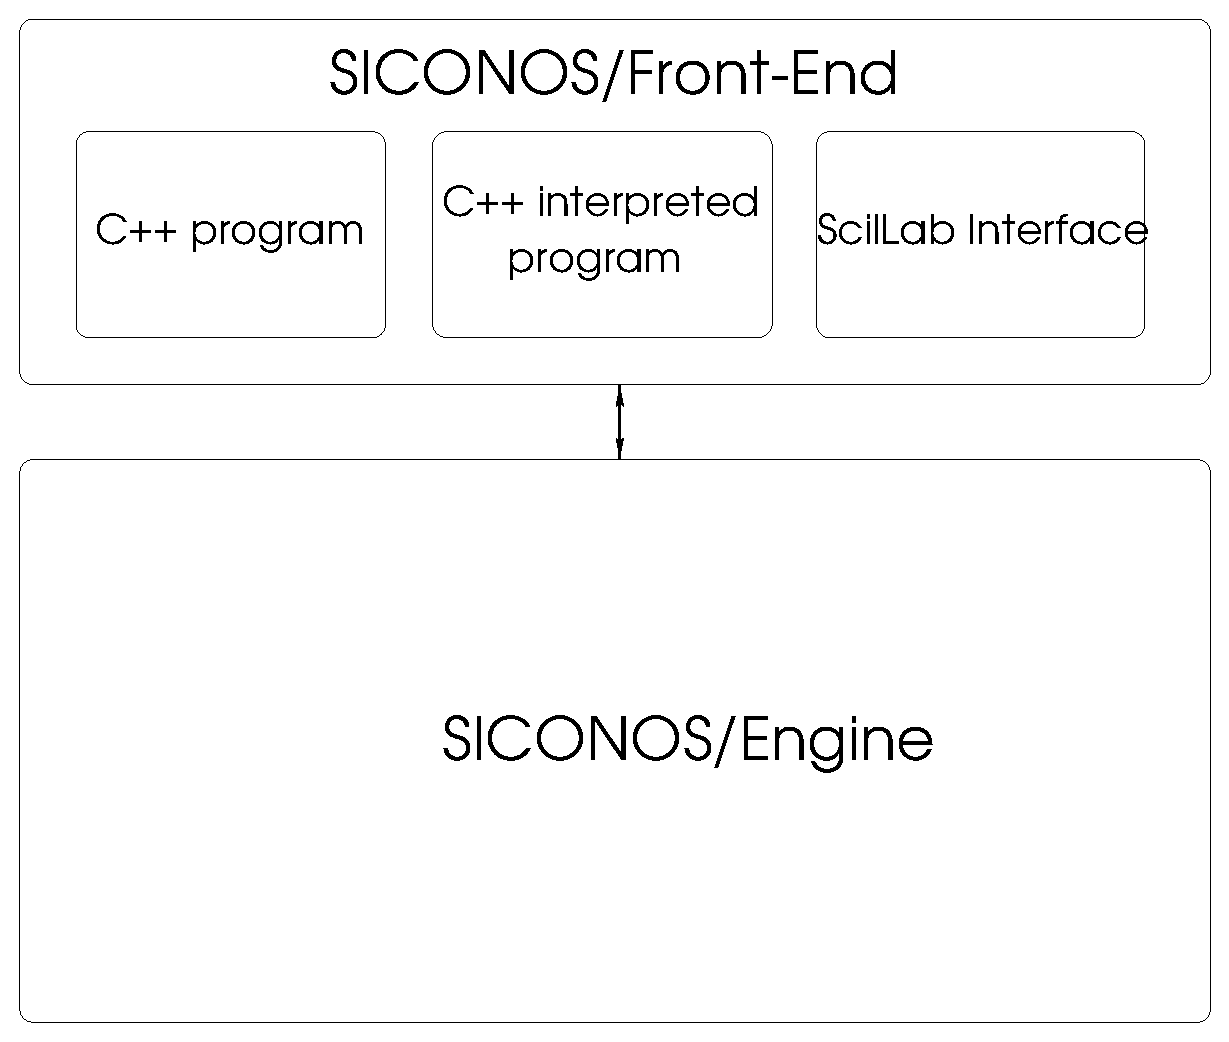
\includegraphics[scale=0.7]{figure/interfaces_scheme.eps}
\end{center}

\subsection{Native C++ interface: \acs{api} C++ }
The first interface will be written in C++. This \acs{api} C++ will contain :
\begin{itemize}
\item all of the public methods or functions of the \acs{engine}
\item a additional set of high level C++ methods in order to provide a macro language to drive the platform. 
\end{itemize}

This \ac{api} could be used in two different ways :
\begin{itemize}
\item compiled directly in an other application or a main file,
\item interpreted trough an C++ interpreter (e.g. Cint).
\end{itemize}


\subsubsection{Compiled C++ program}
%% \begin{ndr}
%% je n'etais pas d'accord avec ce qu'il y avait avant !!
%% le mecanisme d'acces dont vous parliez me semblait antinomique avec la notion
%% de programmation objet. Eventuellement on peut definir une classe debug qui soitami de tout et qui permette d'avoir une certaine visibilite mais ca reste du debug. En exploitation il faut imperativement respecter l'interface sinon c'est le bordel et alors autant faire du basic !
%% f. dubois
%% a completer
%% \end{ndr}


%\subsubsection{Interpreted C++ program}
%This way to launch a simulation is a little bit different from a compiled program. In fact, there is no compilation before running the program, but the program is only interpreted by an other program (Cint) which is linked with the platform. 

%An interpreted C++ program will have the same ability than a compiled C++ program.

\subsection{Interface with \acs{xxxlab}}
The interface through a scientific computation software will be the easiest way to use the computation platform. For example in
\ac{scilab}, the library corresponding to the platform would have to be loaded, and then the high level functions are available to the user.

\ac{scilab} will use functions especially designed for this software. That is to say some functions and objects of the \ac{engine} will
be created and used by calling high level functions which will be known by \ac{scilab}.

This type of interface will produce finally \ac{xxxlab} toolboxes.


\newpage
%---------------------------------------------------------------------------%
\chapter{Conceptual System design}
\label{Sec:ADD-ConceptualSystemDesign}
\section{Analysis and design methods}
For the design of the software, several methods will be introduced. We give in the section \ref{Sec:ADD-DesignMethod} some general informations on the design method which will be used, and in the section \ref{Sec:ADD-ModelTool} a brief overview of the models and tools which will be used.

\subsection{Design methods}
\label{Sec:ADD-DesignMethod}


\subsubsection{\acs{sasd} method}
The \ac{sasd} method allows us to determine the global architecture of the application. Based on the first
specification of the architecture the finest design will be progressive. 
The \ac{sd} method is an extension to the \ac{sa} method. This method is based on the data flow to get a first level
architecture. Then this architecture is evaluated and restructured.

With the \ac{sasd} method, we can evaluate the cohesion and the links between modules which are very important for the evolution of the software.
The architecture  must garanty low links between the different modules and have a high cohesion.


\subsubsection{\acs{uml}}
The \ac{uml} help us to describe using numerous representation the architecture and its use. It allows us to define and check the architecture of our platform.

%=====
% UML
%Une architecture adapt�e est la cl� de vo�te du succ�s d'un d�veloppement.
%Elle d�crit des choix strat�giques qui d�terminent en grande partie les qualit�s du logiciel (adaptabilit�,
%performances, fiabilit�...).
%=====


\subsection{Models and tools}
\label{Sec:ADD-ModelTool}
To build a good architecture for the platform, we will use various modelling languages and tools. According to the type of information we want to depict, the  appropriate model to formally represent data, functions, and behaviours of our system is chosen. Among them, we can cite the following diagrams :
\begin{itemize}
	\item \ac{sasd} method

	\begin{itemize}
		\item Data flow diagram of the \ac{sa} method\\
		On this diagram, we represent the input and output of information. We also see the functions, the data storages and the data flows.
		\item Architecture diagram of the \ac{sd} method\\
		This diagram is built with the data flow diagram and follow the seven steps of the method~:
		\begin{itemize}
        		\item Fundamental diagram
	        	\item Refinement of the data flow diagram
	        	\item Determination of the kind of diagram
		        \item Plan of the frontier
        		\item First level architecture
		        \item Systematic building of the architecture
        		\item Evaluation and restructuration of the architecture
		\end{itemize}
	\end{itemize}

\item \acs{uml} diagrams\\
We will use \ac{uml} tools to create \ac{uml} diagrams.
With \ac{uml}, we can modelise a big part of the architecture with the numerous \ac{uml} diagrams we will see further, and with \ac{ocl}.

\begin{itemize}
\item Sequence diagram\\
This diagram shows the links of the different actions we can find in the platform.
It represents the interactions between the entities of the system.

\item State diagram\\
This diagrams aims to represent automatons as state graphs. It shows the changes of state of an object or a
module in response to the interactions.

%======
%Ce diagramme sert � repr�senter des automates d'�tats finis, sous forme de graphes d'�tats, reli�s par des arcs 
%orient�s qui d�crivent les transitions.
%Les diagrammes d'�tats-transitions permettent de d�crire les changements d'�tats d'un objet ou d'un composant,
%en r�ponse aux interactions avec d'autres objets/composants ou avec des acteurs.
%Un �tat se caract�rise par sa dur�e et sa stabilit�, il repr�sente une conjonction instantan�e des valeurs des
%attributs d'un objet.
%Une transition repr�sente le passage instantan� d'un �tat vers un autre.
%======

\item Collaboration diagram\\
This diagram shows the interactions between the objects (instances of classes and actors). It allows to represent
the context of an interaction.

%====
%Les diagrammes de collaboration montrent des interactions entre objets (instances de classes et acteurs).
%Ils permettent de repr�senter le contexte d'une interaction, car on peut y pr�ciser les �tats des objets qui 
%interagissent.
%====

\item Classes diagram\\
These diagram are collections of classes which show the structure of a model. We use several diagrams for complex models.

%====
%Un diagramme de classes est une collection d'�l�ments de mod�lisation statiques (classes, paquetages...), qui 
%montre la structure d'un mod�le.
%Un diagramme de classes fait abstraction des aspects dynamiques et temporels.  
%Pour un mod�le complexe, plusieurs diagrammes de classes compl�mentaires doivent �tre construits.
%====
\end{itemize}


\item \acs{ocl}\\
It's a language used to describe the invariants in \ac{uml} models. \ac{ocl} is used with the various \ac{uml} diagrams.

%====
%OCL permet de d�crire des invariants dans un mod�le, sous forme de pseudo-code : 
%       pr� et post-conditions pour une op�ration, 
%       expressions de navigation, 
%       expressions bool�ennes, etc...
%====
\end{itemize}


\section{Decomposition description}
The software components should be summarised. These components can be organised in various ways to provide the
views needed by the different members of the development team. The following views present the software
design.

\subsection{Decomposition view}
Here, we show the functional decomposition of the components. It consists in a list of components summarised~:
 
\begin{itemize}
        \item Model formalisation package\\
        This package regroups formalisation methods to modelise a \ac{nsds}. It has to enter data in the data structure of the platform according to the chosen \ac{nsds} using specific plug-ins.
        
        \item Numerical Strategy package\\
        This package represents the computation center of the platform. It uses the entered data to make computations, using \ac{numerics}, and an output plug-in.
        
        \item Input/Output/Plug-ins package\\
        The plug-ins are libraries linked to the platform to increase the flexibility. The input/output plug-in 
	will be used by the previous packages. This plug-in will be at first an \ac{xml} input/output plug-in.
        
        \item Front-end package\\
        Finally, the front-end package is the user part of the platform. So it's closely linked to the platform, at the highest level.
        
\end{itemize}

\subsection{Dependency view}
In this section, we will see the relationship among the components.
\begin{figure}[!hbp]
\begin{center}
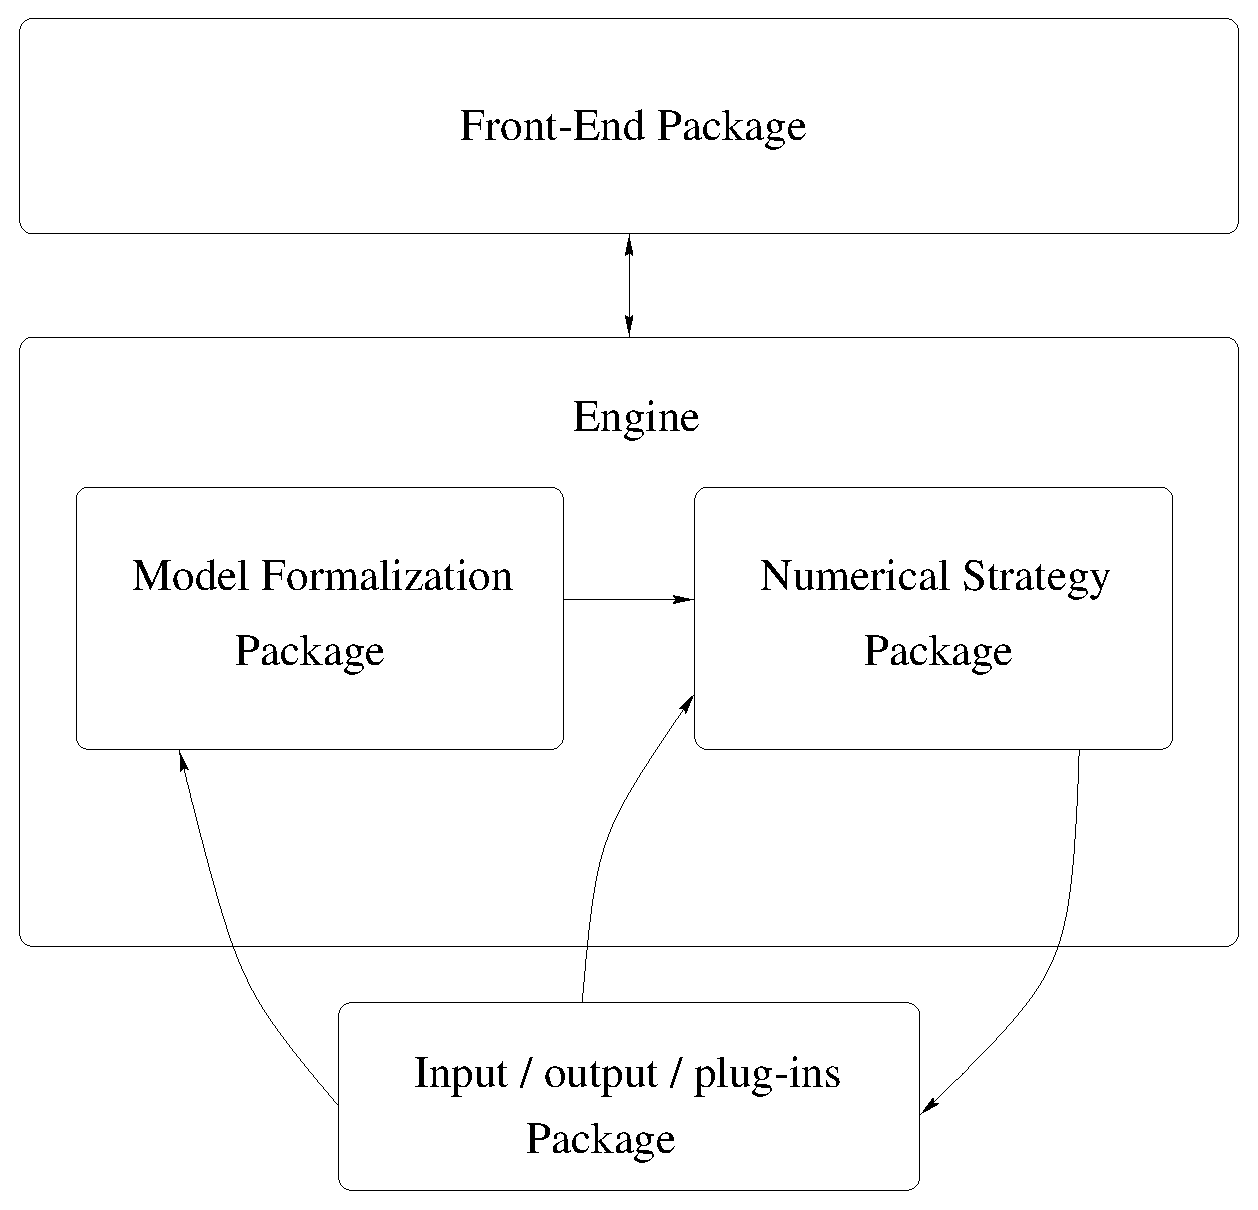
\includegraphics[scale=0.80]{figure/dependency.eps}
\caption{Structure chart of the dependencies}
\label{dependency}
\end{center}
\end{figure}

%\clearpage

The chart \ref{dependency} shows the links seen previously. The Front-end access the platform to drive a complete simulation. The model formalisation uses input methods (basic input method or input method form a dedicated plug-in) to get data, then other
methods to fill the data structure of the platform according to the specificities of each \ac{nsds}.
The numerical strategy uses the model built before to make the computations and an output method (basic output method or output method form a dedicated plug-in) to save the output data.\\

The following diagrams (\ref{sequence_diag1} \& \ref{sequence_diag2}) describe the unfolding of a simulation.
\begin{figure}[!hbp]
\begin{center}
\includegraphics[scale=0.65, bb=30 40 300 775,angle=-90, clip]{figure/sequence1.ps}
\caption{Sequence diagram - Without plug-in}
\label{sequence_diag1}
\end{center}
\end{figure}

\begin{figure}[!hbp]
\begin{center}
\includegraphics[scale=0.65, bb=30 40 330 775,angle=-90, clip]{figure/sequence2.ps}
\caption{Sequence diagram - With plug-in}
\label{sequence_diag2}
\end{center}
\end{figure}

\subsection{Interface view}
We will define in this section the functionalities of the components and their interfaces. 
% It should define the system using one or more of the identity, functions and interface parts of the component description. Suitable methods of presentation are interface files and parameter tables. The intended readership of this description comprises designers, programmers and testers, who need to know how to use the components in the system.
For each communication between components, the information in transit is detailed :
\begin{itemize}

        \item Front-End to Engine\\
        Input files name, matrices, systems, relations that the users want to use for the computations.

        \item Engine to Front-End\\
        Error messages, control messages (``Simulation finished'', indications about the current computation, \dots), some of the simulation result.
        
        \item Model Formalisation to Numerical Strategy\\
        Formalised model, which is composed of several equations (dynamical equation, relations and non smooth laws).
        Most of the equations are composed of matrix.
        
        \item Input/Output/Plug-ins to Model Formalisation\\
        Description of the physical problem. Reading of dedicated files by plug-ins or input/output methods.
        
        \item Plug-ins to Numerical Strategy\\
        Selection of the right methods for computations.
        
        \item Numerical Strategy to Input/Output/Plug-ins\\
        Description of the physical problem at the end or during the simulation.

\end{itemize}

\section{System architecture diagram with related description}
The figure \ref{archi} shows the system architecture using the SA method.
\begin{figure}[p]
\begin{center}
\includegraphics[angle=90, height=22cm]{figure/archi.pstex}
\caption{System architecture - SA diagram}
\label{archi}
\end{center}
\end{figure}
We can see in this figure, the different packages of the architecture.
At first, the package regrouping the input/output modules are represented in light blue and the plug-in modules are represented in dark blue.
In green we see the Front-end package.
In yellow, the Model formalisation package.
In pink, we see the numerical strategy.
Finally, the last module, "update state" is shared between the formalisation and the numerical
strategy package.\\

The diagram \ref{archi_sd} represents the structure we build with the SA diagram. This is the SD diagram.
The one who see is the restructured diagram.
\begin{figure}[p]
\begin{center}
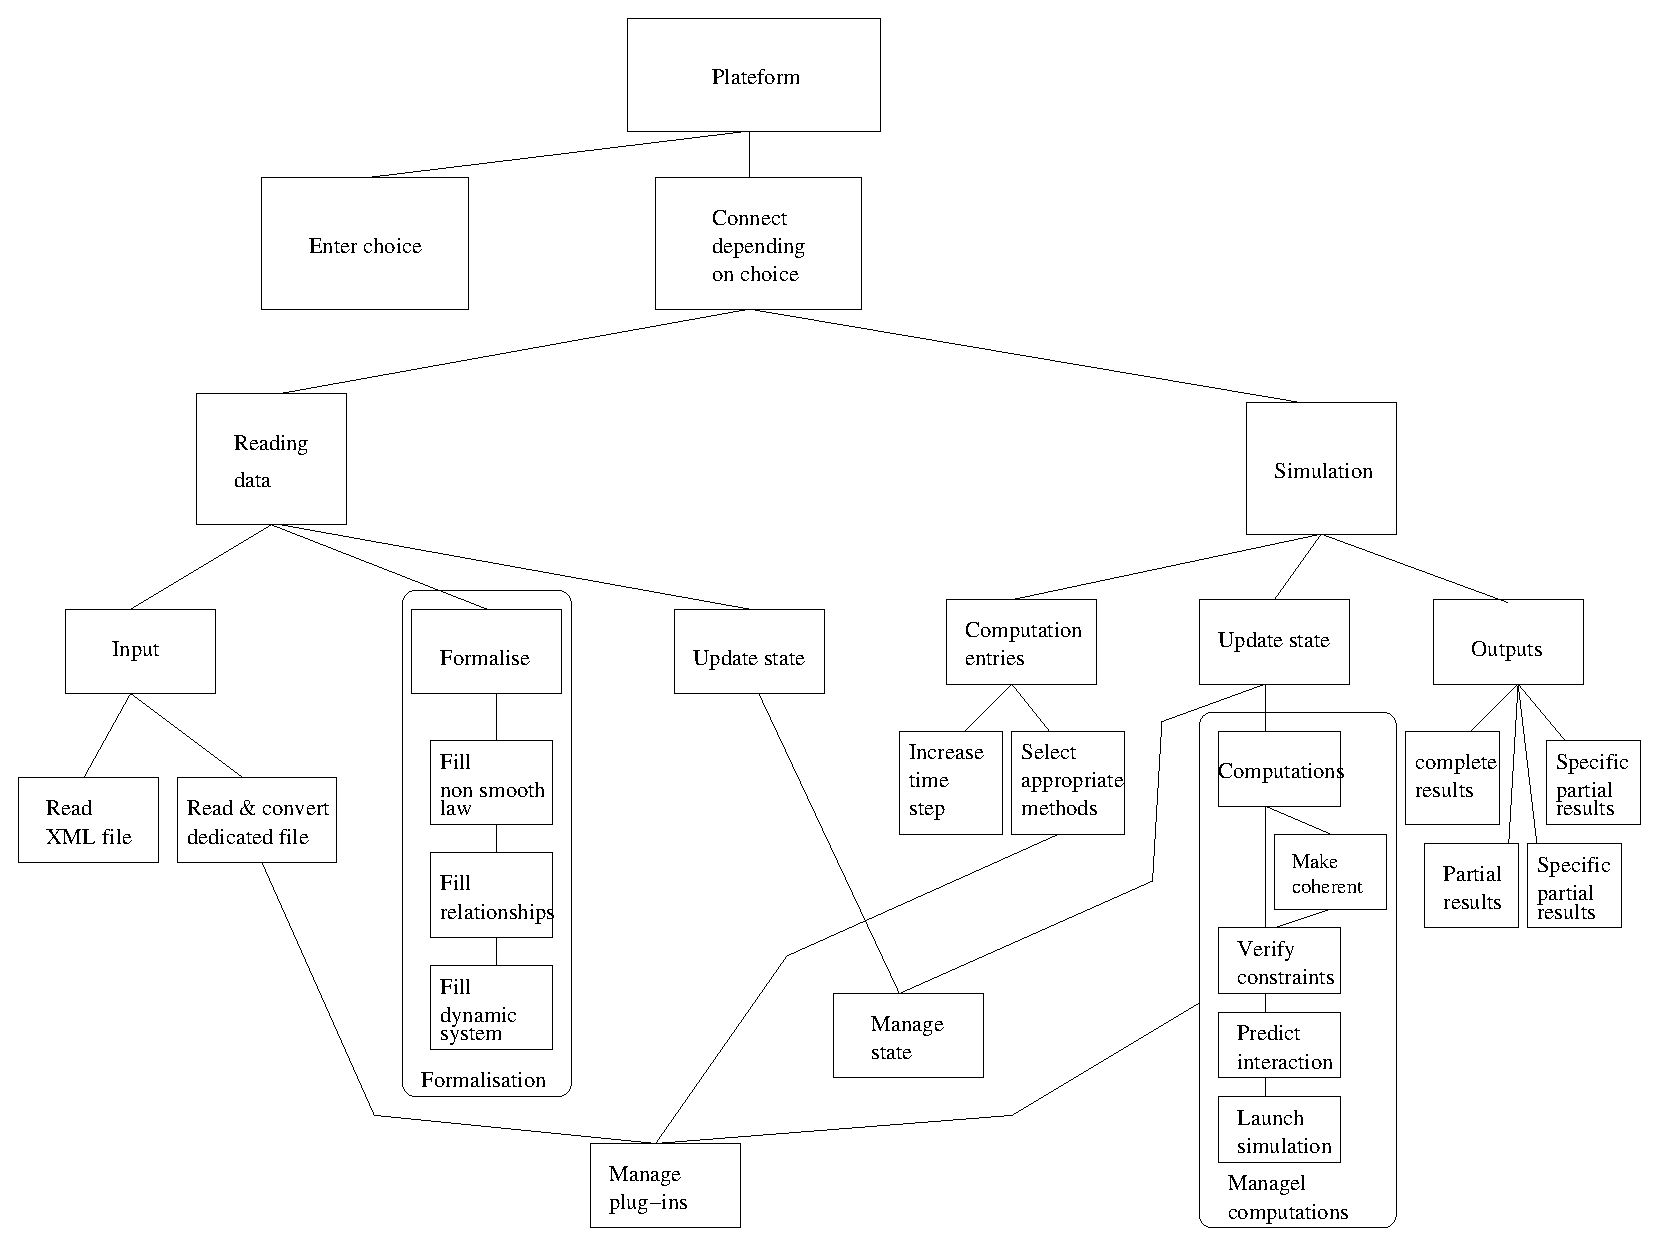
\includegraphics[angle=90, height=22cm]{figure/archi_sd.eps}
\caption{System architecture - SD diagram}
\label{archi_sd}
\end{center}
\end{figure}


\section{SASD conclusion}
The different groups we have made are high cohesion modules because they regroup specific traitments.
During the Detailed Design Phase, we must be carefull with the coupling between these modules.




\newpage
%---------------------------------------------------------------------------%
\chapter{Component description}
\label{Sec:ADD-ComponentDescription}
\section{\ac{lapack}}
It consists in routines for solving systems of simultaneous linear equations, least-squares solutions of linear systems of equations, eigenvalue problems, and singular value problems. The associated matrix factorizations (LU, Cholesky, QR, SVD, Schur, generalized Schur) are also provided, as are related computations such as reordering of the Schur factorizations and estimating condition numbers. Dense and banded matrices are handled, but not general sparse matrices. In all areas, similar functionality is provided for real and complex matrices, in both single and double precision.

\section{MP solver pack}
%\begin{ndr}
%	tell what we'll find in MP solver pack, the Primal Relay, DR, CFP, CFD, ...\\
%	put here some parts of the \ac{tm}
%\end{ndr}

For more details you can refer to the \ac{tm}.

\subsection{Definition of a \acs{lcp} problem}
Let $M$ be a given $n\times n$ matrix, and let $q$ be a given $n$ vector. The linear complementary problem is to find vectors $z$ and $w$ such that
\begin{eqnarray}
M z - w = q \label{equi}\\
z \ge 0, w \ge 0\label{comp}\\
z \cdot w = 0 \label{pdt}
\end{eqnarray}
%
Here, $(z_{i},w_{i})$ is a pair of complementary variables. A solution $(z,w)$ to the above system is called a complementary basic feasible solution if $(z,w)$ is a feasible%
\footnote{A numerical vector that satisfies all the constraints and restrictions in the problem is said a feasible solution.}
solution to $($\ref{equi}$)$ and $($\ref{comp}$)$ and if one variable of the pair $(z_{i},w_{i})$ is  basic% 
\footnote{Consider the following system of linear equality constraints 
\begin{eqnarray}
A x = b \label{basis} \\
x \geq 0
\end{eqnarray}
where $A$ is a given matrix of order $m\times n$ and $m$ is the rank of $A$.
A basis B for \ref{basis} is a square matrix consisting of $m$ columns of A which is nonsingular; and the column vector of variables $x_{B}$ associated with the columns in $B$, arranged in the same order, is the basic vector corresponding to it.
} 
for $i=1,..,n.$




\subsection{Definition of a \acs{cp} problem}
The aim of generalized Non--smooth Newton methods is to provide numerical solutions of systems of nonsmooth equations of the form :
\begin{eqnarray}
  \label{eq:1}
  H(x)=0
\end{eqnarray}
where $H:\Omega \subset \RR^n \mapsto \RR^n $ is locally Lipschitz on the open set $\Omega$. 

If the function $H$ is differentiable on $\Omega$, classical Newton  methods and its variants may be used to solve the equation \eqref{eq:1} and several theorem of local convergence may be formulated. The non differentiability of $H$ gives rise to a lot of complications that invalidates the classical methods.




\subsection{Definition of a Relay problem}
The relay system can be written as a LCP by introducing extra variables. It is convenient to express a standard LCP using the convex analysis formalism:
$$0\le z \perp w \ge 0 \iff -w \in \partial\psi_{[0,+\infty[}(z)$$
Consequently a relay system is synthetically written as follows:
\begin{eqnarray}
Mz-w=q\label{relequi}\\
-w \in \partial\psi_{[-s,s]}(z)\label{relcomp} 
\end{eqnarray}

By extension the set $[-s,s]$ is considered for vector valued problems as the cartesian product of intervals,\\
$$ [-s,s]=\prod_{i=1}^{n}[-s_{i},s_{i}]$$
Set $w^+$ and $w^-$ the positive part and the negative part of $w$, $w=w^+-w^-$ with $w^+=max(w,0)$, $w^-=max(-w,0)$. We introduce two extra variables defined as follows:\\
$z^{p}=s+z ; z^{m}=s-z $ such that $z^{p}+z^{m}=2s$\\


\subsection{Solving routines}
MP solver pack provides solvers for the previous problems. In the one hand, the basics \ac{lcp} solvers for \ac{lcp} problems, and in the other hand extended solvers for \ac{pr}, \ac{dr}, \ac{cfp}, \ac{cfd} problems.



\section{\ac{ode} pack}
It consists of nine solvers, namely a basic solver called LSODE and eight variants of it -- LSODES, LSODA, LSODAR, LSODPK, LSODKR, LSODI, LSOIBT, and LSODIS. The collection is suitable for both stiff and nonstiff systems.  It includes solvers for systems given in explicit form, dy/dt = f(t,y), and also solvers for systems given in linearly implicit form,  A(t,y) dy/dt = g(t,y).  Two of the solvers use general sparse matrix solvers for the linear systems that arise.  Two others use iterative (preconditioned Krylov) methods instead of direct methods for these linear systems.  The most recent addition is LSODIS, which solves implicit problems with general sparse treatment of all matrices involved.



\newpage
%---------------------------------------------------------------------------%
\chapter{Architecture implementation : methods and softwares}
\label{Sec:ADD-ComponentImplementation}
\textit{This chapter precises methods and softwares who will be used to
implement the criticals points of the conceptual architecture described in the before chapters.}

\section{Plugin method}
A simple prototype named BPP has been developped to validate some functionnalities used by the plugins mechanism, like dynamic loading of libraries or
instantiation of objects encapsulated in a dynamic library. This prototype was also needed to verify portability of the libraries. \\
Another point tried with success was the possibility during the instanciation of a dynamical systems too indicate to the platform which computation method
(stored in a given library) has to be used. For example, for a lagrangien system, we can choose a particular function to compute the mass, etc. \\
The next step is to put together this prototype and XML functionnalities in a new prototype to validate our general idea of the functionning of our software.

\section{Fortran encapsulation}

In the \ac{srd}, Corba has been chosen to allow to re-use functions/libraries of other softwares (like \ac{lmgc90}). After a study, it appears that it is possible to make communication between C++ and Fortran languages (a Corba distribution exists), but it is not free. Consequently, to make a LMGC plugin, who may be implemented in the first version of the platform (see \ac{op}), a wrapper will be used.


%\section{C++ interpretor}
% description, pouqruoi on l'a choisi, portabilit�
%A way to use the computation's platform is to write a program in C++ and to run it without compiling it. In order to do that, a C++ interpretor is needed. \ac{cint} is the most famous C++ interpretor found
%on the web. We must insure that \ac{cint} answers our waitings.

\textbf{\ac{cint} specifications}
\begin{description}
	\item[Portability :] \ac{cint} works on number of operating systems. Linux, HP-UX, SunOS, Solaris,
	Windows-NT/95/98/Me, MacOS and with number of compilers, g++, HP-CC/aCC, Sun-CC/CC5, IBM-xlC,
	Compac-cxx, SGI-CC, Visual-C++, Borland-C++.
	\item[Features :] \ac{cint} covers about 95\% of ANSI C and 85\% of C++, supports the STL, allow to
	use embedded compiled C/C++ library code as shared objects.
	\item[Limitations :] \ac{cint} is not as powerfull as a C++ compiler. No "typedef" could be done, no
	overloading for operators, support of an old version of the STL.
\end{description}

A prototype as been created to test the abilities of \ac{cint}. The use of static libraries, templates, and
the STL in a prototype as shown that they can be used if libraries have simple headers (the use of
"makecint" is adviced), the templates are simple and if we use basic functions of the STL.



\section{\acs{xml} files management}

In order to manage the \ac{xml} files (data input/output), the LibXML2 library have been chosen.\\

LibXML2 is an \ac{xml} C parser and toolkit developed for the Gnome project (but usable outside of the Gnome platform). It is a free software available under MIT License. \\

\textbf{Why LibXML2?}

\begin{itemize}
\item Portability : LibXML2 is known to be very portable, the library should build and work without serious troubles on a variety of systems (Linux, Unix, Windows, MacOS, MacOS X, RISC Os,
 ...) ;
\item LibXML2 passes all 1800+ tests from the \ac{oasis} XML Tests Suite ;
\item Diversity : several APIs are implemented by LibXML2 like \ac{dom} or \ac{sax} ;

\end{itemize}

About the use and possibilities of LibXML2, it seems to be adapted and powerfull enought for our project : a prototype verifing, reading, and writing \ac{xml} files has been developed, and the
results are encouraging. The library has only a negative point : modules, methods and structures are summarily documented/specified.

\section{\acs{lmgc90} plugin}
\ac{lmgc90} is an existing software for mechanical computations. The aim of this plugin is to use theirs complex contact detection functions, so that only low level external methods are used. Simulation mechanisms don't change. It consists in communications between the \acs{kernel} and the \ac{lmgc90} plugin. 



\newpage
%---------------------------------------------------------------------------%
%\chapter{Logical validation and verification}
%\label{Sec:ADD-LogicalValidation}
%The logical validation and verification phase refers to the \ac{pti} document.


%\newpage
%---------------------------------------------------------------------------%


%\printglosstex(glo)[p]
\printglosstex(acr)[p]


\listoffigures
%\listoftables
%\cleardoublepage
%\bibliographystyle{plainnat}
%\bibliography{./Biblio/String,./Biblio/Cp.bib,./Biblio/Optim.bib,./Biblio/Contact.bib,./Biblio/NonSmooth.bib,./Biblio/Leger.bib,./Biblio/Petri.bib}
\cleardoublepage
\end{document} 
